\chapter{Analyse des données}

\section{Troubles mentaux, et évolution de leur prise en charge}

    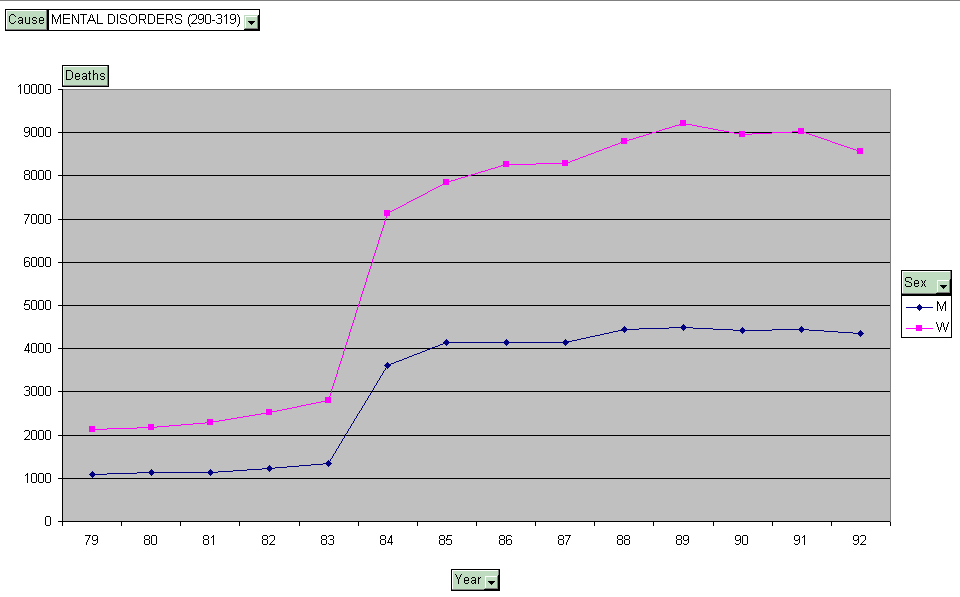
\includegraphics[scale=0.5]{images/mental_disorder.png}

    Une cause de mort a attiré notre attention plus que les autres~: les ``mental disorder''. En plus de présenter une grande disparité
    entre morts chez les hommes et les femmes, le nombre morts causées par ces troubles a drastiquement augmenté en 1983.

    Nous avons essayé de chercher des signes d'une augmentation aussi drastique des morts chez les autres causes, en vain. Il était donc
    clair que cette augmentation était bien spécifique aux \textit{troubles mentaux}.

    Nous sommes donc allés chercher les événements marquants s'étant produits en Grande-Bretagne autour de 1983, et quelques recherches
    et articles plus tard, nous avons isolé la cause à l'origine de cette hausse : le \href{en.wikipedia.org/wiki/Mental_Health_Act_1983‎}{Mental Health Act of 1983}.

    Cet acte parlementaire a introduit une nouvelle classification des \textit{troubles mentaux} et un traitement

\section{Morts néonatales et nouveaux certificats de décès}

    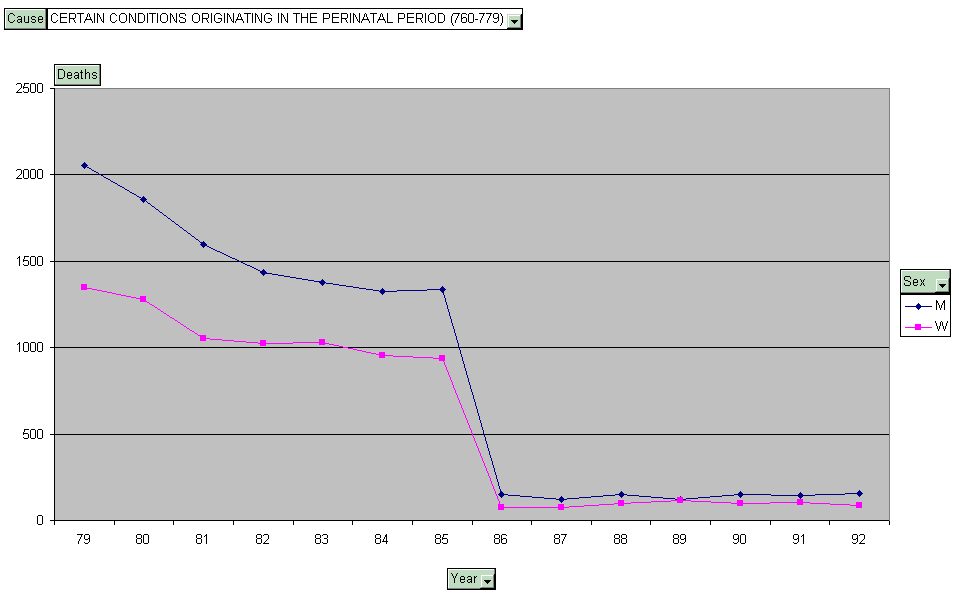
\includegraphics[scale=0.5]{images/perinatal.png}

    Blah blah.

\section{Maladies musculo-squelettique}

    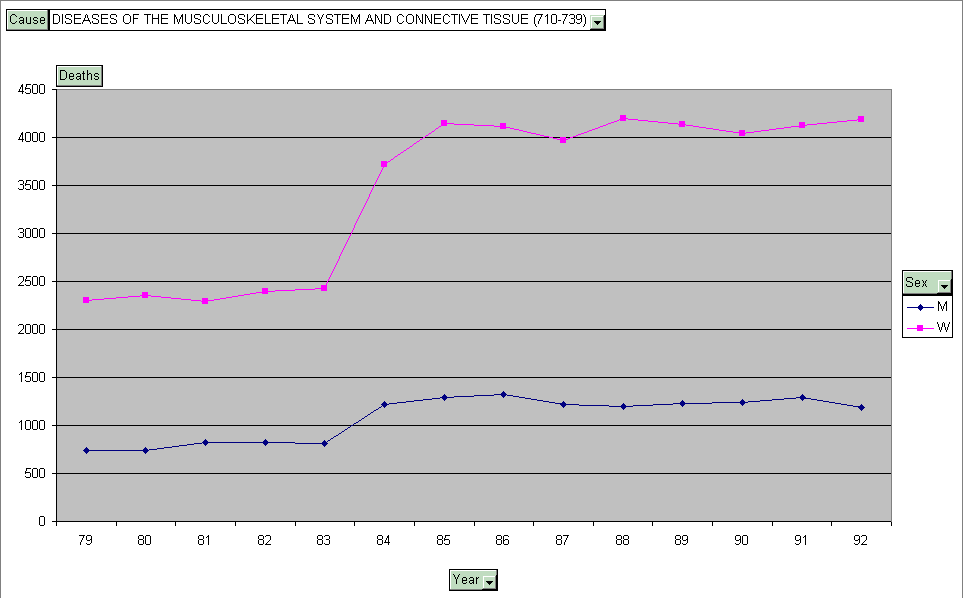
\includegraphics[scale=0.5]{images/muscoskeletal.png}

    Blah blah.